El anonimato no es una cosa que sólo interese a los usuarios que navegan por internet, sino que nosotros podemos querer montar un servidor en internet que permanezca anónimo para las personas que lo usen. Este punto del problema es uno de los más complejos de resolver dentro de la red Tor.\\
Un usuario que desee montar un servicio oculto dentro de la red Tor montará un nodo normal dentro de la red y dentro del fichero de configuración indicará que es un servicio oculto. Esta configuración hace que dicho nodo no sirva para redirección de tráfico y en lugar de esto se le redirige el tráfico cuando un usuario quiera acceder al servicio.\\
Para la comunicación entre un usuario y el proveedor del servicio oculto se utilizan dos tipos de conceptos: puntos introductorios y nodos rendezvous.\\
Cuando el servicio es montado y arrancado lo primero que hace es buscar tres puntos distribuidos de manera equitativa dentro de la red. Estos puntos son los llamados puntos introductorios. La clave de que el servicio oculto permanezca anónimo recae sobre estos puntos introductorios. Cuando un usuario quiera pedir el servicio se le facilitará desde dentro de la red Tor el nodo introductorio más fácil de acceder para su máquina. Con este nodo podrá acordar con el servicio el siguiente paso de la comunicación.\\
Una vez hecha la petición o $"handshake"$ entre el usuario y el servicio estos dos acuerdan un nodo dentro de la red llamado rendezvous. Una vez acordado dicho nodo el sericio oculto crea un circuito dentro de la red que conecte en el otro extremo con el nodo rendezvous, el usuario realiza el mismo proceso. Esto lo que ha generado es un circuito que une al servicio con el usuario sin que ninguno de los dos se conozcan entre sí. El circuito sería algo como:\\ 
$Usuario\Leftrightarrow Guard\Leftrightarrow Relay\Leftrightarrow Rendezvous\Leftrightarrow Relay\Leftrightarrow Guard \Leftrightarrow Servicio \ oculto$\\
Al no salir este circuito fuera de la red Tor no se requiere del uso de nodos de salida.\\
Para el funcionamiento de los servicios ocultos conviene saber cómo están organizados por dentro tanto los nodos comunes como los servicios ocultos.\\
Esta organización recae sobre una tabla hash que hace que los nodos y servicios se distribuyan de manera equitativa dentro de la red. La intención de esto es que no sobrecarguemos siempre a los mismos nodos o que haya servicios ocultos más accesibles que otros.
\begin{figure}[h]
	\centering
	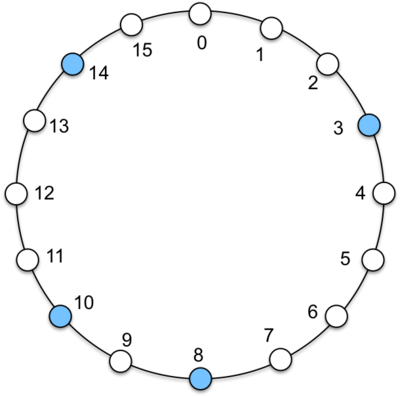
\includegraphics[scale=0.5]{dht-chord-ring.png}
	\caption{Tabla Hash distribuida.}
\end{figure}\\
En la figura por ejemplo se observan como nodos los círculos pequeños. Aquellos que están en azul podrían representar los nodos que son puntos introductorios para algún servicio. Como se observa están bien distribuidos y cubren de manera uniforme el espacio.\\
Para que la red sea lo más dinámica posible y difícil de monitorizar se hace que todas estas posiciones que se le asignan tanto a los nodos como a los servicios ocultos cambien cada 24 horas lo que hace que un nodo o servicio a lo largo de su vida difícilmente esté en una posición en la que ya haya caído previamente.\\
Se estima que hay unos 80 mil servicios ocultos dentro de la red Tor pero sólo 8 mil de ellos son permanentes. La razón de esto es que la mayoría de ellos están dedicados a actividades ilegales o a comunicación entre miembros de bandas organizadas y permanecen la mayoría del tiempo offline para sólo conectarse cuando requieren de comunicación o de ofrecer sus servicios a alguien. Esto hace que sea difícil su vigilancia ya que cambia tanto su posición dentro de la red Tor como su link .onion y sus puntos introductorios.